\documentclass[aspectratio=169]{beamer}
\usetheme{Madrid}
\usecolortheme{default}

\usepackage[utf8]{inputenc}
\usepackage[T1]{fontenc}
\usepackage{graphicx}
\usepackage{tikz}
\usepackage{listings}
\usepackage{xcolor}
\usepackage{hyperref}
\usepackage{amsmath}
\usepackage{amssymb}

% Code listing settings
\lstset{
    basicstyle=\ttfamily\footnotesize,
    breaklines=true,
    frame=single,
    numbers=left,
    numberstyle=\tiny,
    keywordstyle=\color{blue},
    commentstyle=\color{green!60!black},
    stringstyle=\color{red},
    backgroundcolor=\color{gray!10}
}

% Custom colors
\definecolor{edgeblue}{RGB}{0,114,178}
\definecolor{edgegreen}{RGB}{0,158,115}
\definecolor{edgeorange}{RGB}{230,159,0}

\title{Edge Server Project}
\subtitle{Complete System Architecture and Implementation}
\author{Edge Computing Team}
\date{\today}
\institute{Edge Server Ubuntu}

\begin{document}

\begin{frame}
\titlepage
\end{frame}

\begin{frame}{Table of Contents}
\tableofcontents
\end{frame}

\section{Project Overview}

\begin{frame}{What is the Edge Server Project?}
\begin{itemize}
    \item \textbf{Complete IoT Edge Computing Solution}
    \item \textbf{Vehicle Telemetry Processing System}
    \item \textbf{Real-time Data Collection and Visualization}
    \item \textbf{Self-contained Network Infrastructure}
\end{itemize}

\vspace{1cm}
\begin{center}
%\includegraphics[width=0.6\textwidth]{edge-computing-diagram}
\end{center}
\end{frame}

\begin{frame}{System Architecture Overview}
\begin{center}
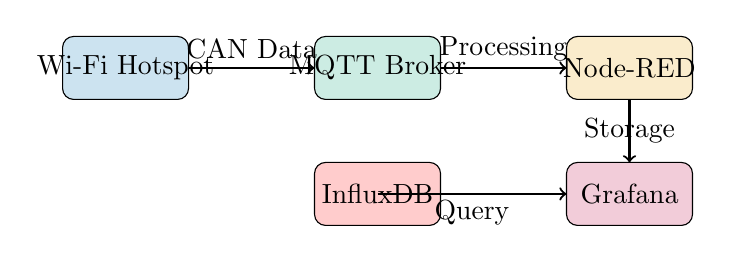
\begin{tikzpicture}[scale=0.8]
    % Hotspot
    \draw[fill=edgeblue!20, rounded corners] (0,4) rectangle (2,5) node[pos=0.5] {Wi-Fi Hotspot};
    
    % MQTT
    \draw[fill=edgegreen!20, rounded corners] (4,4) rectangle (6,5) node[pos=0.5] {MQTT Broker};
    
    % Node-RED
    \draw[fill=edgeorange!20, rounded corners] (8,4) rectangle (10,5) node[pos=0.5] {Node-RED};
    
    % InfluxDB
    \draw[fill=red!20, rounded corners] (4,2) rectangle (6,3) node[pos=0.5] {InfluxDB};
    
    % Grafana
    \draw[fill=purple!20, rounded corners] (8,2) rectangle (10,3) node[pos=0.5] {Grafana};
    
    % Arrows
    \draw[->, thick] (2,4.5) -- (4,4.5);
    \draw[->, thick] (6,4.5) -- (8,4.5);
    \draw[->, thick] (9,4) -- (9,3);
    \draw[->, thick] (5,2.5) -- (8,2.5);
    
    % Labels
    \node at (3,4.8) {CAN Data};
    \node at (7,4.8) {Processing};
    \node at (9,3.5) {Storage};
    \node at (6.5,2.2) {Query};
\end{tikzpicture}
\end{center}
\end{frame}

\section{Hotspot Implementation}

\begin{frame}{Wi-Fi Hotspot: Why is it needed?}
\begin{columns}
\column{0.6\textwidth}
\begin{itemize}
    \item \textbf{Standalone Network}
    \begin{itemize}
        \item Independent of external networks
        \item Controlled environment for IoT devices
    \end{itemize}
    \item \textbf{Device Connectivity}
    \begin{itemize}
        \item Vehicles can connect directly
        \item Sensors and edge devices access
    \end{itemize}
    \item \textbf{Internet Sharing}
    \begin{itemize}
        \item Connected devices get internet access
        \item Remote management capabilities
    \end{itemize}
\end{itemize}

\column{0.4\textwidth}
\begin{center}
%\includegraphics[width=0.8\textwidth]{hotspot-diagram}
\end{center}
\end{columns}
\end{frame}

\begin{frame}{Hotspot: How it was implemented}
\begin{columns}
\column{0.5\textwidth}
\textbf{Network Configuration:}
\begin{itemize}
    \item SSID: EdgeServerHotspot
    \item Password: strongpass123
    \item IP Range: 192.168.12.0/24
    \item Gateway: 192.168.12.1
    \item DHCP: 192.168.12.10-50
\end{itemize}

\column{0.5\textwidth}
\textbf{Technical Components:}
\begin{itemize}
    \item NetworkManager (nmcli)
    \item dnsmasq (DHCP server)
    \item iptables (NAT routing)
    \item IP forwarding enabled
\end{itemize}
\end{columns}

\vspace{0.5cm}
\begin{center}
\begin{lstlisting}[language=bash]
#!/bin/bash

# Auto-detect Wi-Fi interface
WIFI_IF=$(nmcli device status | grep wifi | awk '{print $1}')

if [ -z "$WIFI_IF" ]; then
  echo "No Wi-Fi interface found. Exiting."
  exit 1
fi

# Configuration
SSID="EdgeServerHotspot"
PASSWORD="strongpass123"
INTERNET_IF=$(nmcli device status | grep connected | grep ethernet | awk '{print $1}')
HOTSPOT_IP="192.168.12.1"
SUBNET="192.168.12.0"
RANGE_START="192.168.12.10"
RANGE_END="192.168.12.50"
NETMASK="255.255.255.0"

echo "Using Wi-Fi interface: $WIFI_IF"
echo "Sharing internet from: $INTERNET_IF"
\end{lstlisting}
\end{center}
\end{frame}

\section{Docker and Containers}

\begin{frame}{Why Docker is needed?}
\begin{columns}
\column{0.6\textwidth}
\begin{itemize}
    \item Service Isolation
    \begin{itemize}
        \item Each service runs independently
        \item No conflicts between dependencies
    \end{itemize}
    \item Portability
    \begin{itemize}
        \item Easy deployment across environments
        \item Consistent runtime environment
    \end{itemize}
    \item Scalability
    \begin{itemize}
        \item Services can be scaled individually
        \item Resource allocation control
    \end{itemize}
    \item Management
    \begin{itemize}
        \item Centralized orchestration
        \item Easy service updates and rollbacks
    \end{itemize}
\end{itemize}

\column{0.4\textwidth}
\begin{center}
%\includegraphics[width=0.8\textwidth]{docker-architecture}
\end{center}
\end{columns}
\end{frame}

\begin{frame}{Docker Compose Architecture}
\begin{center}
\begin{lstlisting}[language=yaml]
services:
  mqtt:
    image: eclipse-mosquitto
    container_name: mosquitto
    ports:
      - "1883:1883"
    volumes:
      - ./mosquitto/config:/mosquitto/config
      - ./mosquitto/data:/mosquitto/data
      - ./mosquitto/log:/mosquitto/log

  nodered:
    image: nodered/node-red
    container_name: nodered
    ports:
      - "1880:1880"
    volumes:
      - nodered_data:/data
      - csv_data:/csv
    depends_on:
      - mqtt
      - influxdb
    user: "1000:1000"

  influxdb:
    image: influxdb:1.8
    container_name: influxdb
    ports:
      - "8086:8086"
    volumes:
      - influxdb_data:/var/lib/influxdb
    environment:
      - INFLUXDB_DB=edge_data
      - INFLUXDB_HTTP_AUTH_ENABLED=true
      - INFLUXDB_ADMIN_USER=admin
      - INFLUXDB_ADMIN_PASSWORD=admin123
\end{lstlisting}
\end{center}

\textbf{Key Features:}
\begin{itemize}
    \item \textbf{Volume Management}: Persistent data storage
    \item \textbf{Service Dependencies}: Proper startup order
    \item \textbf{Port Mapping}: External access to services
    \item \textbf{Environment Variables}: Configuration management
\end{itemize}
\end{frame}

\section{Individual Services}

\subsection{MQTT Broker (Mosquitto)}

\begin{frame}{MQTT: Message Queuing Telemetry Transport}
\begin{columns}
\column{0.6\textwidth}
\textbf{Purpose:}
\begin{itemize}
    \item Lightweight messaging protocol
    \item Real-time data transmission
    \item IoT device communication
    \item Publish/subscribe pattern
\end{itemize}

\textbf{Configuration:}
\begin{itemize}
    \item Port: 1883
    \item Anonymous access enabled
    \item Persistent storage
    \item File-based logging
\end{itemize}

\column{0.4\textwidth}
\begin{center}
\begin{lstlisting}[language=text]
persistence true
persistence_location /mosquitto/data/
log_dest file /mosquitto/log/mosquitto.log
listener 1883
allow_anonymous true
\end{lstlisting}
\end{center}
\end{columns}
\end{frame}

\subsection{Node-RED}

\begin{frame}{Node-RED: Visual Programming Interface}
\begin{columns}
\column{0.6\textwidth}
\textbf{Key Functions:}
\begin{itemize}
    \item \textbf{CSV Processing}: Parse incoming data files
    \item \textbf{CAN Decoding}: Vehicle-specific message interpretation
    \item \textbf{Data Transformation}: Format for storage
    \item \textbf{Flow Control}: Route data between services
\end{itemize}

\textbf{Processing Pipeline:}
\begin{enumerate}
    \item Receive CSV via MQTT
    \item Parse and validate data
    \item Decode CAN messages
    \item Store in InfluxDB
    \item Generate decoded CSV
\end{enumerate}

\column{0.4\textwidth}
\begin{center}
%\includegraphics[width=0.8\textwidth]{nodered-flow}
\end{center}
\end{columns}
\end{frame}

\begin{frame}{Node-RED: CAN Data Decoding}
\textbf{Supported CAN Messages:}
\begin{itemize}
    \item \textbf{CAN ID 0x101}: Cylinder Pressure (MPa)
    \item \textbf{CAN ID 0xD7}: Vehicle Speed (km/h)
\end{itemize}

\vspace{0.5cm}
\begin{lstlisting}[language=javascript]
// Fixed Decode CAN Data Function for Node-RED
// Handles both CSV strings and parsed object arrays
// Validates rows and formats data safely for InfluxDB

let rows = msg.payload;
let decoded = [];
let influxData = [];

// Debug input
node.log('Input type: ' + typeof rows);
node.log('Input length: ' + (Array.isArray(rows) ? rows.length : 'not array'));

// Case 1: Payload is raw CSV string
if (typeof rows === 'string') {
    let lines = rows.split('\\n').filter(line => line.trim() !== '');
    
    lines.forEach((line, index) => {
        if (line.includes('timestamp') || line.includes('CANID') || line.includes('CANDATA')) {
            node.log('Skipping header line: ' + line);
            return;
        }
        
        let parts = line.split(',');
        if (parts.length < 3) return;
        
        let ts = parseFloat(parts[0]);
        let id = String(parts[1] || '').toLowerCase();
        let data = String(parts[2] || '');
        
        if (isNaN(ts) || !id || !data || data.length < 8) {
            node.log('Skipping invalid CSV row ' + index + ': ' + line);
            return;
        }
        
        // Process CAN ID 0x101 (Cylinder Pressure)
        if (id === "101") {
            let raw = ((bytes[3] << 2) | (bytes[4] >> 6)) & 0x3FF;
            let value = raw * 0.02;
            decoded.push({ Timestamp: ts, CANID: id, Label: "CylinderPressure", Value: value, Unit: "Mpa" });
        }
    });
}

// Outputs
msg.payload = decoded;
msg.topic = "csv_output";
return [msg, { payload: influxData }];
\end{lstlisting}
\end{frame}

\subsection{InfluxDB}

\begin{frame}{InfluxDB: Time-Series Database}
\begin{columns}
\column{0.6\textwidth}
\textbf{Why InfluxDB?}
\begin{itemize}
    \item \textbf{Time-Series Optimized}
    \begin{itemize}
        \item Efficient timestamp storage
        \item Fast time-based queries
    \end{itemize}
    \item \textbf{IoT Data Handling}
    \begin{itemize}
        \item High-frequency data ingestion
        \item Compression and retention policies
    \end{itemize}
    \item \textbf{Performance}
    \begin{itemize}
        \item Sub-second query response
        \item Efficient storage utilization
    \end{itemize}
\end{itemize}

\column{0.4\textwidth}
\textbf{Configuration:}
\begin{itemize}
    \item Port: 8086
    \item Database: edge\_data
    \item Admin: admin/admin123
    \item User: edgeuser/edgepass
\end{itemize}
\end{columns}
\end{frame}

\subsection{Grafana}

\begin{frame}{Grafana: Data Visualization Platform}
\begin{columns}
\column{0.6\textwidth}
\textbf{Capabilities:}
\begin{itemize}
    \item \textbf{Real-time Dashboards}
    \begin{itemize}
        \item Live vehicle telemetry
        \item Configurable refresh rates
    \end{itemize}
    \item \textbf{Historical Analysis}
    \begin{itemize}
        \item Time-range selection
        \item Trend analysis
    \end{itemize}
    \item \textbf{Alerting}
    \begin{itemize}
        \item Threshold-based notifications
        \item Multiple notification channels
    \end{itemize}
\end{itemize}

\column{0.4\textwidth}
\begin{center}
%\includegraphics[width=0.8\textwidth]{grafana-dashboard}
\end{center}
\end{columns}
\end{frame}

\begin{frame}{Grafana: Dashboard Configuration}
\textbf{Pre-configured Panels:}
\begin{itemize}
    \item \textbf{Cylinder Pressure}: Real-time pressure monitoring
    \item \textbf{Vehicle Speed}: Speed tracking over time
    \item \textbf{Data Quality}: Validation and error tracking
\end{itemize}

\vspace{0.5cm}
\begin{lstlisting}[language=yaml]
apiVersion: 1

datasources:
  - name: InfluxDB
    type: influxdb
    access: proxy
    url: http://influxdb:8086
    database: edge_data
    user: admin
    secureJsonData:
      password: admin123
    jsonData:
      httpMethod: POST
      httpHeaders:
        - name: Authorization
          value: Basic YWRtaW46YWRtaW4xMjM=
      version: InfluxQL
      timeInterval: 5s
\end{lstlisting}
\end{frame}

\section{Deployment and Management}

\subsection{Deploy Script}

\begin{frame}{Automated Deployment Script}
\begin{columns}
\column{0.6\textwidth}
\textbf{Deployment Process:}
\begin{enumerate}
    \item \textbf{Wi-Fi Hotspot Setup}
    \item \textbf{Grafana Configuration}
    \item \textbf{Docker Container Deployment}
    \item \textbf{Service Verification}
    \item \textbf{Browser Automation}
\end{enumerate}

\textbf{Key Features:}
\begin{itemize}
    \item One-command deployment
    \item Error handling and validation
    \item Automatic service startup
    \item User-friendly output
\end{itemize}

\column{0.4\textwidth}
\begin{center}
\begin{lstlisting}[language=bash]
#!/bin/bash

set -e

echo "Setting up Wi-Fi hotspot..."
cd "$(dirname "$0")/hotspot"
chmod +x setup-full-hotspot.sh
sudo ./setup-full-hotspot.sh

cd ../grafana
chmod +x setup-grafana.sh
./setup-grafana.sh

echo "Deploying Docker containers..."
cd ../docker

# Check Docker
if ! command -v docker &> /dev/null; then
  echo "Docker not installed. Please install Docker and try again."
  exit 1
fi
sudo systemctl restart docker

# Start Docker Compose stack
sudo docker compose up -d
\end{lstlisting}
\end{center}
\end{columns}
\end{frame}

\subsection{Cleanup Script}

\begin{frame}{System Cleanup and Restoration}
\begin{columns}
\column{0.6\textwidth}
\textbf{Cleanup Process:}
\begin{enumerate}
    \item \textbf{Remove Hotspot}
    \item \textbf{Restore NetworkManager}
    \item \textbf{Stop Docker Services}
    \item \textbf{Clean System Changes}
    \item \textbf{Data Preservation Options}
\end{enumerate}

\textbf{System Restoration:}
\begin{itemize}
    \item iptables rules removal
    \item dnsmasq configuration restore
    \item IP forwarding disable
    \item Network interface restoration
\end{itemize}

\column{0.4\textwidth}
\begin{center}
\begin{lstlisting}[language=bash]
#!/bin/bash
WIFI_IF=$(nmcli device status | grep wifi | awk '{print $1}')
echo "Cleaning up Edge Server..."

# REMOVE HOTSPOT CONNECTION
HOTSPOT_NAME="EdgeServerHotspot"
echo "Removing NetworkManager hotspot: $HOTSPOT_NAME"
nmcli con delete "$HOTSPOT_NAME" 2>/dev/null || echo "No hotspot connection to delete"

# RESTORE NetworkManager
echo "Re-enabling NetworkManager control on wlan0..."
nmcli dev set $WIFI_IF managed yes

# REMOVE DNSMASQ CONFIG
if [ -f /etc/dnsmasq.conf.backup ]; then
  echo "Restoring original dnsmasq.conf..."
  sudo mv /etc/dnsmasq.conf.backup /etc/dnsmasq.conf
else
  echo "dnsmasq.conf.backup not found - skipping restore"
fi

echo "Stopping and disabling dnsmasq..."
sudo systemctl stop dnsmasq
sudo systemctl disable dnsmasq
\end{lstlisting}
\end{center}
\end{columns}
\end{frame}

\section{Data Flow Architecture}

\begin{frame}{Complete Data Flow Diagram}
\begin{center}
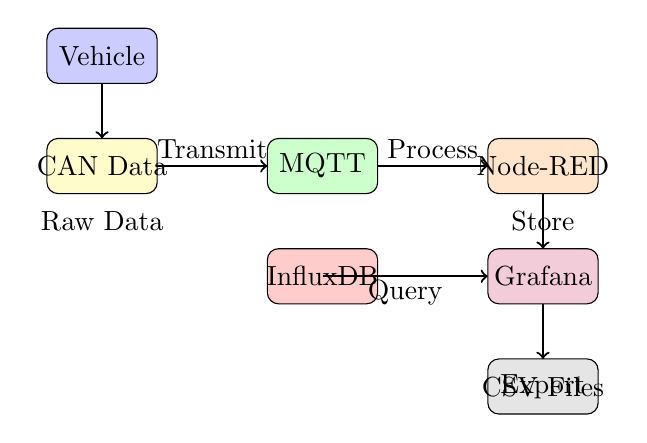
\begin{tikzpicture}[scale=0.7]
    % Vehicle
    \draw[fill=blue!20, rounded corners] (0,6) rectangle (2,7) node[pos=0.5] {Vehicle};
    
    % CAN Data
    \draw[fill=yellow!20, rounded corners] (0,4) rectangle (2,5) node[pos=0.5] {CAN Data};
    
    % MQTT
    \draw[fill=green!20, rounded corners] (4,4) rectangle (6,5) node[pos=0.5] {MQTT};
    
    % Node-RED
    \draw[fill=orange!20, rounded corners] (8,4) rectangle (10,5) node[pos=0.5] {Node-RED};
    
    % InfluxDB
    \draw[fill=red!20, rounded corners] (4,2) rectangle (6,3) node[pos=0.5] {InfluxDB};
    
    % Grafana
    \draw[fill=purple!20, rounded corners] (8,2) rectangle (10,3) node[pos=0.5] {Grafana};
    
    % CSV Output
    \draw[fill=gray!20, rounded corners] (8,0) rectangle (10,1) node[pos=0.5] {CSV Files};
    
    % Arrows
    \draw[->, thick] (1,6) -- (1,5);
    \draw[->, thick] (2,4.5) -- (4,4.5);
    \draw[->, thick] (6,4.5) -- (8,4.5);
    \draw[->, thick] (9,4) -- (9,3);
    \draw[->, thick] (5,2.5) -- (8,2.5);
    \draw[->, thick] (9,2) -- (9,1);
    
    % Labels
    \node at (1,3.5) {Raw Data};
    \node at (3,4.8) {Transmit};
    \node at (7,4.8) {Process};
    \node at (9,3.5) {Store};
    \node at (6.5,2.2) {Query};
    \node at (9,0.5) {Export};
\end{tikzpicture}
\end{center}
\end{frame}

\section{Key Benefits and Advantages}

\begin{frame}{System Benefits}
\begin{columns}
\column{0.5\textwidth}
\textbf{Technical Advantages:}
\begin{itemize}
    \item \textbf{Edge Computing}
    \begin{itemize}
        \item Local data processing
        \item Reduced latency
        \item Offline operation
    \end{itemize}
    \item \textbf{Scalability}
    \begin{itemize}
        \item Modular architecture
        \item Easy service addition
        \item Resource optimization
    \end{itemize}
\end{itemize}

\column{0.5\textwidth}
\textbf{Operational Benefits:}
\begin{itemize}
    \item \textbf{Reliability}
    \begin{itemize}
        \item Container isolation
        \item Automatic restart
        \item Fault tolerance
    \end{itemize}
    \item \textbf{Flexibility}
    \begin{itemize}
        \item Easy modifications
        \item Plugin architecture
        \item Custom dashboards
    \end{itemize}
\end{itemize}
\end{columns}
\end{frame}

\section{Use Cases and Applications}

\begin{frame}{Practical Applications}
\begin{columns}
\column{0.6\textwidth}
\textbf{Vehicle Telemetry:}
\begin{itemize}
    \item \textbf{Real-time Monitoring}
    \begin{itemize}
        \item Engine performance
        \item Fuel efficiency
        \item Safety systems
    \end{itemize}
    \item \textbf{Data Analysis}
    \begin{itemize}
        \item Predictive maintenance
        \item Driver behavior
        \item Fleet optimization
    \end{itemize}
\end{itemize}

\column{0.4\textwidth}
\textbf{Industrial IoT:}
\begin{itemize}
    \item Sensor data collection
    \item Equipment monitoring
    \item Process optimization
    \item Quality control
\end{itemize}
\end{columns}
\end{frame}

\section{Conclusion}

\begin{frame}{Summary}
\begin{center}
\textbf{Complete Edge Computing Solution}
\end{center}

\vspace{0.5cm}
\begin{itemize}
    \item \textbf{Self-contained Network}: Wi-Fi hotspot with internet sharing
    \item \textbf{Containerized Services}: MQTT, Node-RED, InfluxDB, Grafana
    \item \textbf{Automated Deployment}: One-command setup and cleanup
    \item \textbf{Real-time Processing}: Vehicle CAN data analysis
    \item \textbf{Data Visualization}: Interactive dashboards and monitoring
    \item \textbf{Scalable Architecture}: Easy to extend and modify
\end{itemize}

\vspace{1cm}
\begin{center}
\textbf{Ready for Production Deployment}
\end{center}
\end{frame}

\begin{frame}{Questions and Discussion}
\begin{center}
\Large \textbf{Thank You!}
\vspace{1cm}

\large Questions and Discussion
\end{center}
\end{frame}

\end{document}
